% !Mode:: "TeX:UTF-8"

\chapter{绪论}

\section{研究背景及意义}
CPU (Central Processing Unit) 是一台计算机最重要最核心的组成部分,也叫做中央处理器。处理器设计制造也一直是高精尖的技术领域。自2020年美国开始禁止向中国出口高端芯片以来,使得芯片成为了这两年的热点话题,我国更加注重处理器设计领域的发展,推出了一系列相关政策推动我国加快发展自己的芯片设计和制造产业。其中以龙芯为首的多家国内企业多年以来也一直不断地在相关领域内投入研发。

目前市场上的处理器大多使用的是x86和ARM指令集架构,其中x86处理器主要是Intel和AMD这两家美国公司占主流,主打产品是一些高性能计算机的处理器;ARM公司主要靠指令架构的授权来盈利,ARM架构的处理器广泛的使用在各种嵌入式产品和终端中,在现在万物互联的趋势下普及到生活的各个角落中。这两个架构几乎垄断了处理器的市场,如果有一家企业想要设计制造一款处理器,无法避免的需要到x86或者ARM的指令集授权,支付一笔昂贵的费用,极大提高了芯片的成本。

而RISC-V的出现打破了这一局面,RISC-V是2010年始于美国加州大学伯克利分校的一款开源指令集架构,与大多数指令集相比,RISC-V指令集没有高昂的授权费用,任何人都可以使用RISC-V设计和制造芯片,而不用支付任何费用。这极大的降低了芯片的成本。同时由于这是一个年轻的指令集架构,没有x86和ARM由于需要兼容老旧的设计而带来的历史包袱,RISC-V使用了更先进的模块化设计理念。因此RISC-V一经面世,就受到了业内的关注和支持,尤其是在受到美国制裁的前提下,RISC-V非常适合我国的国情,我国的许多企业都加入了RISC-V基金会,在RISC-V基金会的19位高级成员中,有11位都是中国企业。

% \begin{figure}[htb]
% 	\centering
% 	\setlength\tabcolsep{3pt}  % 同一行中的图片间隔
% 	\vspace{5pt} % 图片上部的空白,如果太小的话,图片顶部会与正文内容十分接近
% 	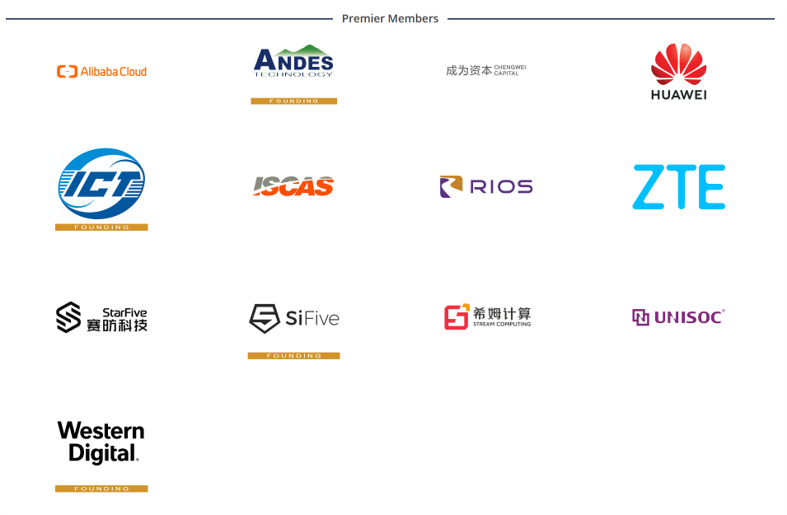
\includegraphics[width=1\textwidth]{RISC-V_Foundation_Members.png}
% 	\caption{RISC-V 基金会高级成员(评委老师说这张图要删掉)}
% 	\label{fig:figure1}
% \end{figure}

早期的RISC-V由于还在逐渐发展,大家对其仍然抱着观望的态度,主要还是用在一些功能比较简单的嵌入式芯片设计中,使用RISC-V设计的高性能处理器仍然较少,但是近几年来不断有国内的企业开始使用RISC-V设计高性能处理器,例如阿里巴巴的玄铁系列,而中科院计算所也研发了一款开源的RISC-V高性能处理器名为香山,希望能够通过开源香山以及香山的开发流程和工具,带动国内开发者的热情,促进处理器相关领域的发展。而本文的研究就是在香山处理器的开发平台上进行的。

在一个高性能处理器架构里,分支预测是必不可少的一个部件。由于分支指令会导致处理器的指令流水线出现中断,因此一个高效的分支预测部件能够尽可能地减少流水线中断的情况,极大提升处理器的整体性能。由于现代的处理器都在往更高的频率,更深的流水线发展,以期待获得更高的性能。但同时更高的频率也限制了每个流水级间逻辑门级的数量,更深的流水线则造成了更大的分支误预测惩罚。因此对分支预测的设计带来了更大的挑战,即如何在满足频率要求的前提下实现预测算法,并且保证较高的分支预测准确率。

香山处理器第一版的分支预测是参考了加州大学伯克利分校开发的一款开源RISC-V处理器BOOM (The Berkeley Out-of-Order Machine) 的分支预测设计。该分支预测设计有4级流水,使用混合预测器,以TAGE预测器作为主要的预测器。由于设计代码与香山开发使用的是相同的Chisel语言,并且代码开源,因此BOOM能够为香山带来许多的参考思路。

在讨论先进的分支预测算法和设计时,现有的论文大多基于模拟器来建模研究,没有考虑到具体的硬件实现,以及针对高频的优化。在真实的物理设计中,由于硬件特性和时序要求,相对于论文中的设计,在某些地方可能需要做出针对性的修改和优化,才能够将其真正的在硬件上实现。除了BOOM以外,有先进分支预测架构的开源设计也是寥寥无几,只能够通过公司的相关产品介绍和论文中窥到一些细节。因此本文以国内开源RISC-V高性能处理器香山为研究平台,在其第一版架构的基础上对分支预测进行了重构和优化,使其能够达到更高的性能和频率。同时,所有的设计代码都是开源的,能够给RISC-V社区中的开发者们提供借鉴和启发。

\section{国内外研究现状}


\subsection{RISC-V发展现状}
RISC-V是加州大学伯克利分校在2010年首次发布的一个开源指令集架构,这是一个年轻的指令集架构,它是吸收了大量已有指令集,如x86,ARM,MIPS等指令集的设计经验,弥补了它们的不足,做出大量的改进后产生的,并且为了给体系结构领域注入新的活力,RISC-V拥抱开源,使用RISC-V无需支付任何费用,让全世界的开发者能够不受成本政治等边缘因素的影响,全新的投入到RISC-V的设计与开发中来。

除了开源免费以外,RISC-V作为一个全新的指令集架构,不需要考虑历史兼容性的问题,这也使得它能够更加精简,门槛更低,相比于x86和ARM动辄几千页的手册,RISC-V的手册只有寥寥几百页,学习门槛大大降低,开发者们能够在更短的时间内掌握RISC-V设计的基础。

由于多种因素,RISC-V一出世就受到了工业界和学术界的关注与肯定。在经过一段时间的发展与完善后,大家都开始尝试以RISC-V为基础进行研究与设计。大量的研究成果也不断发布,最具代表性的就是加州大学伯克利分校的Rocket和BOOM两款开源的处理器设计,其中BOOM作为开源高性能处理器的代表,更是在大量的论文中作为研究平台和对比对象。而国内也有大量的成果,例如在阿里巴巴2021年9月10日正式开源的玄铁910,就是一款使用RISC-V指令集的处理器。此外国内还有很多公司都有相关的产品,如华米科技的黄山1号、紫光展锐的春藤系列,以及兆易创新的GD32VF103等。

\subsection{分支预测发展现状}

在现在的主流高性能处理器中一般使用的都是混合分支预测器,即将不同的分支预测器混合起来,在不同的情况下分别选择使用不同预测器的预测结果,以达到覆盖更多类型分支,以及满足硬件设计要求的目的。

分支预测器也有着不同的类型,首先是最简单的静态分支预测,静态分支预测通过一些静态的信息来进行预测,而不会考虑指令动态执行时的不同情况,例如可以将所有的分支都预测为不跳转,或者将向后跳转的分支预测为跳转,将向前的分支预测为不跳转。与之对应的就是更复杂,更准确的动态分支预测。动态分支预测能够通过收集程序运行时指令的动态信息来进行训练,学习到分支指令跳转的模式,根据不同情况给出预测,这样能够达到更加高的准确率,当然同时就对预测算法与硬件实现提出了更高的要求。由于更高的预测准确率,因此大部分处理器还是使用动态预测器为主。

此外分支预测器也可以按照使用的分支历史分为局部历史预测器和全局历史预测器。程序执行一段时间后,我们能够得到大量分支指令跳转的历史,通过这些历史对预测器进行训练,找到特定的模式来为后续的分支指令做预测,而局部历史预测器倾向于使用部分的分支历史来做预测,例如循环预测器只会寻找可能是循环跳转指令的分支\cite{barnes2009patchmatch}。而全局历史预测器会倾向于使用所有的分支历史或某种全局分支历史的哈希,例如TAGE预测器。两种类型的预测器都各有优劣,因此将它们混合使用往往可以更好的覆盖不同的分支指令。

这里给出一些处理器的分支预测设计

% \subsection{引用参考文献}
% 在references.bib中添加参考文献对应的bibtex,使用$\backslash$cite\{\}引用论文的id,如引用参考文献\cite{barnes2009patchmatch}。

% \subsection{插入图片}
% 如图\ref{fig:figure1}所示,在文章中插入图片。使用$\backslash$begin\{figure\}插入图片,支持的格式有jpg、png、eps与pdf等,本例使用$\backslash$begin\{tabular\}插入三幅图像(一行三列),如果只插入一副图像则不需使用$\backslash$begin\{tabular\}。

% \begin{figure}[htb]
% 	\centering
% 	\setlength\tabcolsep{3pt}  % 同一行中的图片间隔
% 	\vspace{5pt} % 图片上部的空白,如果太小的话,图片顶部会与正文内容十分接近
% 	\begin{tabular}{ccc}
% 		\includegraphics[width=0.32\textwidth]{baboon.jpg} &
% 		\includegraphics[width=0.32\textwidth]{lena.jpg} &
% 		\includegraphics[width=0.32\textwidth]{parrot.jpg} \\
% 		(a) 图1 & (b) 图2 & (c) 图3 \\[1ex]
% 	\end{tabular}
% 	\caption{图片示例}
% 	\label{fig:figure1}
% \end{figure}

% \subsection{插入公式}
% 如公式\eqref{eq:equation1}所示,为公式示例:
% \begin{equation}
% 	c = a + b
% 	\label{eq:equation1}
% \end{equation}

% \subsection{插入表格}

% 如表格\ref{tb:table1}所示,为表格示例。可以通过"https://www.tablesgenerator.com/"以用户界面形式创建表格,并将表格转化为latex代码。

% \begin{table}[]
% 	\caption{表格标题}
% 	\label{tb:table1}
% 	\centering
% 	\begin{tabular}{|c|c|c|}
% 		\hline
% 		a   & b   & c   \\ \hline
% 		1.1 & 1.2 & 1.3 \\ \hline
% 		1.4 & 1.5 & 1.6 \\ \hline
% 	\end{tabular}
% \end{table}

\section{本文思路及研究方法}

本文首先介绍了开源RISC-V高性能处理器在国内的研究意义,以及为什么选择使用RISC-V来设计处理器的原因,并对香山超标量乱序处理器的基本结构做了介绍。之后进一步介绍了其中分支预测的整体架构,并在此基础上从性能和频率两个方面对其进行了优化。

\subsection{性能方面}

性能方面的优化

\subsection{频率方面}

频率方面的优化

介绍完相关的优化之后,我们使用Design Compiler对整个处理器架构进行了时序评估,并使用Verilator对整体设计进行行为级仿真,运行SPEC2006测试程序,通过分析相关的性能数据用于评估其改进结果。

\section{论文结构}

本文分为以下几个章节,内容安排如下:

第一章的主要内容是介绍了本课题的研究背景和意义,讨论了一些国内外的研究现状,简单介绍了香山处理器的整体架构,并对本文内容做了规划

第二章的主要内容是介绍分支预测架构中的各个预测器及其设计实现细节

第三章的主要内容是提出以FTB为主的限制分支预测宽度的分支预测改进策略

第四章的主要内容是提出以FTQ为主的实现解耦前端取指单元的设计

% 第五章的主要内容是介绍了针对改进分支预测性能做过的部分尝试及其细节

第五章的主要内容是介绍评估测试设计所用到的环境,以及相关的评估指标,统计结果及其分析

第六章的主要内容是对本文工作的一个总结,并指出目前仍然存在的一些问题,对之后的工作做出了展望

